%%%%%%%%%%%%%%%%%%%%%%%%%%%%%%%%%%%%%%%%%%%%%%%%%%%%%%%%%%%%%%%%%%%%%%%%%%%%%%%%%%%%%%%%%%%
%%%%%%%%%%%% Trabalho de final de curso em Eng. de Teleinformatica - UFC %%%%%%%%%%%%%%%%%%
%%%%%%%%%%%%%%%%%%%%%%%%%%%%%%%%%%%%%%%%%%%%%%%%%%%%%%%%%%%%%%%%%%%%%%%%%%%%%%%%%%%%%%%%%%%
%%%%%%%%%%%%%%%%%%%%%%%%%%%%%%%%%% Luiz Camara Neto %%%%%%%%%%%%%%%%%%%%%%%%%%%%%%%%%%%%%%%
%%%%%%%%%%%%%%%%%%%%%%%%%%%%%%%%%%%%%%%%%%%%%%%%%%%%%%%%%%%%%%%%%%%%%%%%%%%%%%%%%%%%%%%%%%%
%%%%%%%%%%%%%%%%%%%%%%%%%%%%%%% RESULTADOS E DISCUSSOES %%%%%%%%%%%%%%%%%%%%%%%%%%%%%%%%%%%
%%%%%%%%%%%%%%%%%%%%%%%%%%%%%%%%%%%%%%%%%%%%%%%%%%%%%%%%%%%%%%%%%%%%%%%%%%%%%%%%%%%%%%%%%%%

\chapter{Resultados e Discuss\~{o}es}
\thispagestyle{empty}

Este cap\'{i}tulo tem por objetivo expor e discutir os resultados obtidos na avalia\c{c}\~{a}o dos m\'{e}todos propostos por \citeauthor{Soares:2006} (\citeyear{Soares:2006}) e \citeauthor{Zana:2001} (\citeyear{Zana:2001}). Al\'{e}m disso, ser\~{a}o apresentadas as duas bases de imagens utilizadas para realizar os experimentos de avalia\c{c}\~{a}o destes m\'{e}todos.

\section{Bases de Imagens}

O paradigma de avalia\c{c}\~{a}o das imagens segmentadas \'{e} a compara\c{c}\~{a}o destas com seus respectivos mapas de refer\^{e}ncia fornecidos por bases de imagens p\'{u}blicas. Para este trabalho, foram utilizadas as imagens de retina e seus mapas de refer\^{e}ncia associados de duas bases de imagens: DRIVE \cite{Niemeijer:2004} and STARE \cite{Hoover:2000}. Cada base possui dois mapas de refer\^{e}ncia associados para cada imagen de retina.

A base DRIVE (\textit{Digital Retinal Images for Vessel Extraction}) \'{e} constitu\'{i}da de 40 imagens de retina de tamanho 565 $\times$ 584 pixels. As imagens foram obtidas de um programa para triagem de retinopatia diab\'{e}tica na Holanda usando a c\^{a}mera \textit{Canon CR5 non-mydriatic 3 charge-couple device (CCD)}  com campo de vis\~{a}o de $45\,^{\circ}$. A base est\'{a} dividida em dois grupos: grupo de treinamento e grupo de teste. Cada grupo \'{e} composto por 20 imagens comprimidas em formato TIFF. Para este trabalho, apenas as imagens do grupo de teste foram usadas.

A base STARE (\textit{STructured Analysis of the REtina}) cont\'{e}m 20 imagens de tamanho 700 $\times$ 605 pixels divididas entre imagens com presen\c{c}a de patologias e imagens livres de agentes patol\'{o}gicos. Essas altera\c{c}\~{o}es tornam a segmenta\c{c}\~{a}o dessas imagens mais disafiadoras de serem realizadas com alta precis\~{a}o. Cada divis\~{a}o possui 10 imagens obtidas usando a c\^{a}mera \textit{TopCon TRV-50} com campo de vis\~{a}o de $35\,^{\circ}$. Todas as imagens desta base foram usadas na avalia\c{c}\~{a}o dos m\'{e}todos.

\section{Resultados e Discuss\~{o}es}

Os resultados obtidos na avalia\c{c}\~{a}o dos m\'{e}todos ser\~{a}o expostos nesta se\c{c}\~{a}o de modo que os mesmos suportem as discuss\~{o}es e conclus\~{o}es deste trabalho. As ilustra\c{c}\~{o}es utilizadas seguem o mesmo padr\~{a}o de cores usado na Figura \ref{Fig:imgresex}. A Tabela \ref{tabcor} ilustra a determina\c{c}\~{a}o do padr\~{a}o de cores a partir da correspond\^{e}ncia pixel a pixel entre a imagem segmentada e o mapa de refer\^{e}ncia. Todos os m\'{e}todos usados para teste foram implementados pelo autor deste trabalho baseado nas especifica\c{c}\~{o}es descritas nos respectivos artigos. 

  \begin{table}[h]
   \caption{Tabela de cores baseada na correspond\^{e}ncia pixel a pixel}
    \label{tabcor}
    \centering
    \scalebox {0.75 }[0.75 ]{ 
      \begin{tabular}{c|cccc}
        \toprule
        Cor & Imagem Segmentada & Mapa de Refer\^{e}ncia \\
        \midrule                 
        $\color{LG} Verde$  &\textbf{Vaso} &\textbf{Vaso} \\
        $\color{LG} Verde$  &N\~{a}o-Vaso &N\~{a}o-Vaso \\
        $\color{LB} Azul$  &\textbf{Vaso} &N\~{a}o-Vaso \\
        $\color{LR} Vermelho$  &N\~{a}o-Vaso &\textbf{Vaso} \\
        \bottomrule
      \end{tabular}
    }
  \end{table}

As Tabelas \ref{tabDRIVE} e \ref{tabRESULTS} apresentam os valores m\'{e}dios para as medidas de informa\c{c}\~{a}o quantitativa para as bases DRIVE e STARE, respectivamente. Observa-se que o desempenho do m\'{e}todo supervisionado proposto por \citeauthor{Soares:2006} (\citeyear{Soares:2006}) \'{e} bem superior ao m\'{e}todo n\~{a}o-supervisionado proposto por \citeauthor{Zana:2001} (\citeyear{Zana:2001}) para quase todos os valores. A \'{u}nica exce\c{c}\~{a}o deve-se ao desempenho superior do m\'{e}todo n\~{a}o-supervisionado na base DRIVE com rela\c{c}\~{a}o \`{a} especificidade. As Figuras \ref{Fig:exemplesDrive} e \ref{Fig:exemplesStare} ilustram o desempenho dos 2  m\'{e}todos de segmenta\c{c}\~{a}o para imagens das bases DRIVE e STARE, respectivamente. As Figuras \ref{Fig:exemplesDrive}(e) e \ref{Fig:exemplesDrive}(f) confirmam o desempenho  dos m\'{e}todos como mostra a Tabela \ref{tabDRIVE}. O menor n\'{u}mero de pixels vermelhos e maior n\'{u}mero de pixels azuis na imagem de compara\c{c}\~{a}o do m\'{e}todo supervisionado confirmam o desempenho superior de sensibilidade e inferior de especificidade deste m\'{e}todo na base utilizada. O n\'{u}mero menor de pixels vermelhos indica que uma maior quantidade de vasos foi segmentada. O maior n\'{u}mero de pixels verdes tamb\'{e}m pode ser utilizado para confirmar a maior coincid\^{e}ncia na segmenta\c{c}\~{a}o dos vasos. O n\'{u}mero maior de pixels azuis indica houve um n\'{u}mero significativo de sobre-segmenta\c{c}\~{a}o na imagem. Ou seja, pixels que n\~{a}o s\~{a}o pertencentes a vasos foram segmentados como pixels de vasos. Observando a Tabela \ref{tabDRIVE}, notamos que o ganho de especificade do m\'{e}todo n\~{a}o-supervisionado \'{e} consideravelmente inferior quando comparado ao ganho de sensibilidade do m\'{e}todo supervisionado. Portanto, \'{e} esperado que a precis\~{a}o do m\'{e}todo supervisionado seja maior. De fato, a Tabela \ref{tabDRIVE} confirma esta expectativa.

\begin{figure}[H]
    \centering
    \subfigure[\label{Fig:imgrgb10Drive}]
        {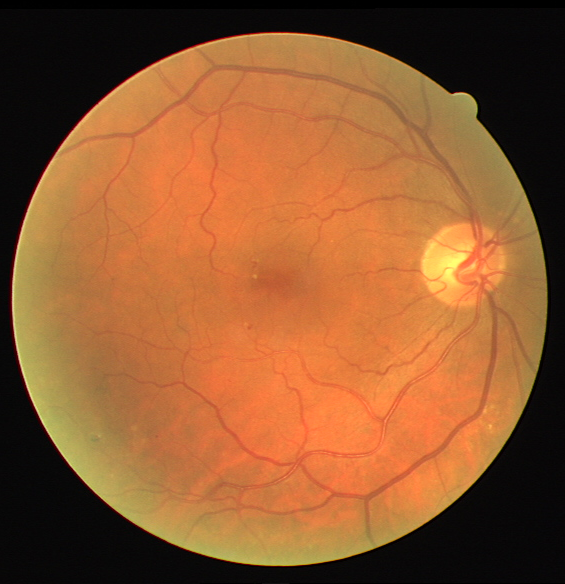
\includegraphics[width=6cm]{Figuras/Cap4/Drive_RGB_1}}
    \subfigure[\label{Fig:imgmanual10Drive}]
        {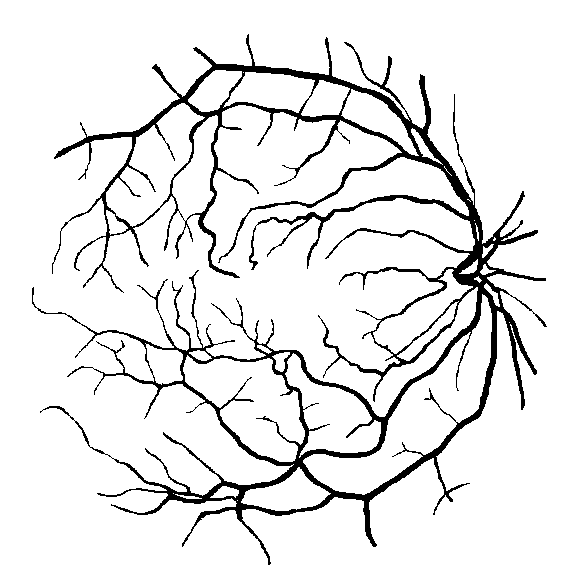
\includegraphics[width=6cm]{Figuras/Cap4/Drive_Manual_10}}
    \subfigure[\label{Fig:imgsoares10Drive}]
        {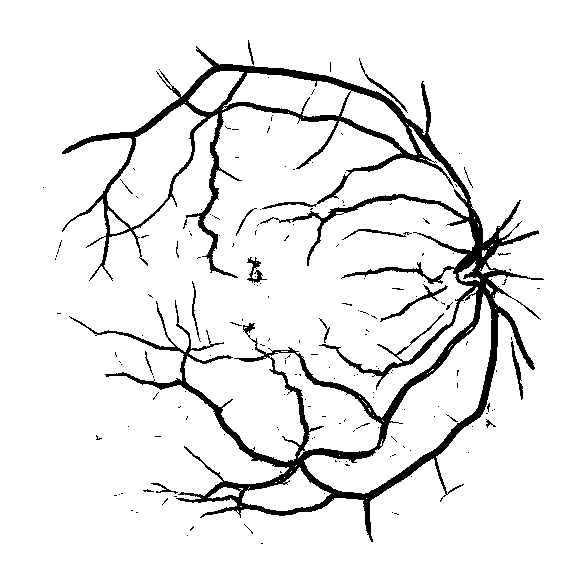
\includegraphics[width=6cm]{Figuras/Cap4/Drive_Soares_10}}
    \subfigure[\label{Fig:imgzana10Drive}]
        {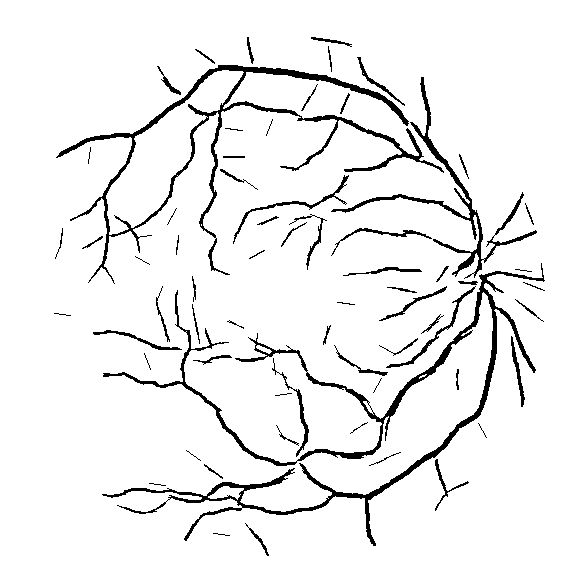
\includegraphics[width=6cm]{Figuras/Cap4/Drive_Zana_10}}
    \subfigure[\label{Fig:imgsoares10manualDrive}]
        {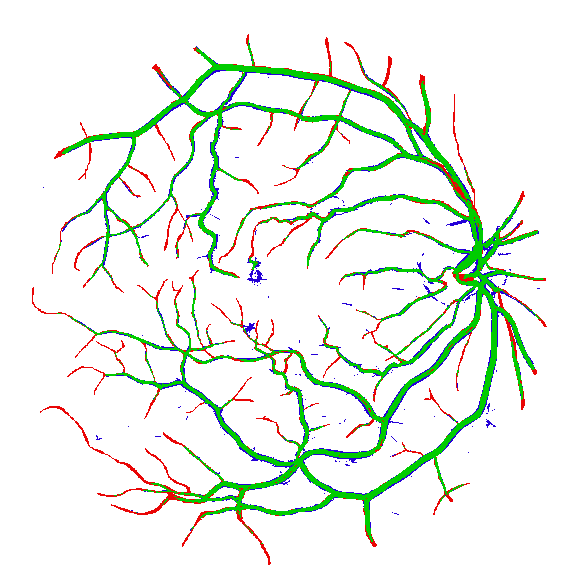
\includegraphics[width=6cm]{Figuras/Cap4/Drive_SoaresxManual_10}}
    \subfigure[\label{Fig:imgzana10manualDrive}]
        {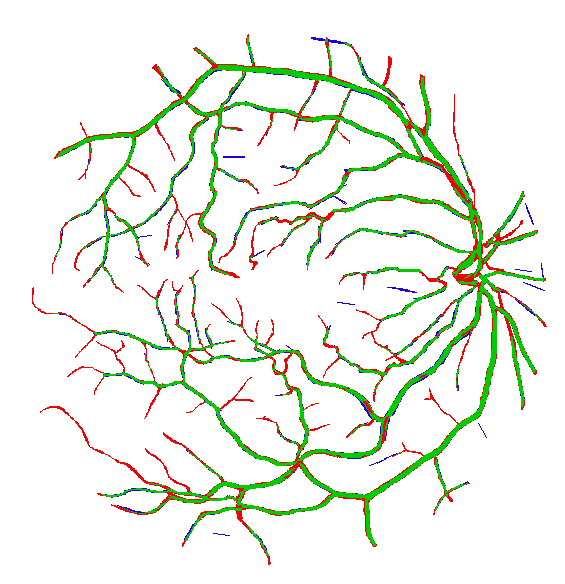
\includegraphics[width=6cm]{Figuras/Cap4/Drive_ZanaxManual_10}}
    \caption{(a) Imagem original (Fonte: Base de Dados DRIVE); (b) Mapa de refer\^{e}ncia (Fonte: Base de Dados DRIVE); (c) Imagem segmentada para o m\'{e}todo supervisionado (Fonte: Pr\'{o}prio Author); (d) Imagem segmentada para o m\'{e}todo n\~{a}o-supervisionado (Fonte: Pr\'{o}prio Author); (e) Imagem de compara\c{c}\~{a}o entre o m\'{e}todo supervisionado e o mapa de refer\^{e}ncia (Fonte: Pr\'{o}prio Author); (f) Imagem de compara\c{c}\~{a}o entre o m\'{e}todo n\~{a}o-supervisionado e o mapa de refer\^{e}ncia (Fonte: Pr\'{o}prio Author).}
    \label{Fig:exemplesDrive}
\end{figure}

\begin{figure}[!h]
    \centering
    \subfigure[\label{Fig:imgrgb1}]
        {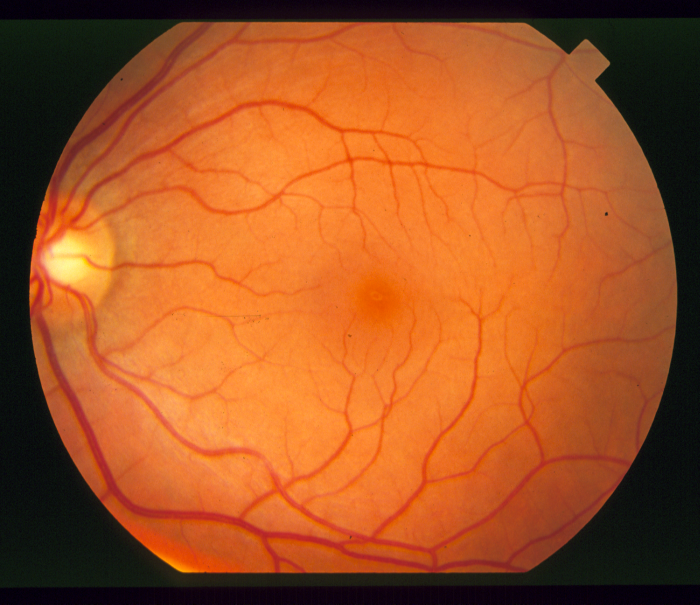
\includegraphics[width=6.4cm]{Figuras/Cap4/Stare_RGB_1}}
    \subfigure[\label{Fig:imgmanual1}]
        {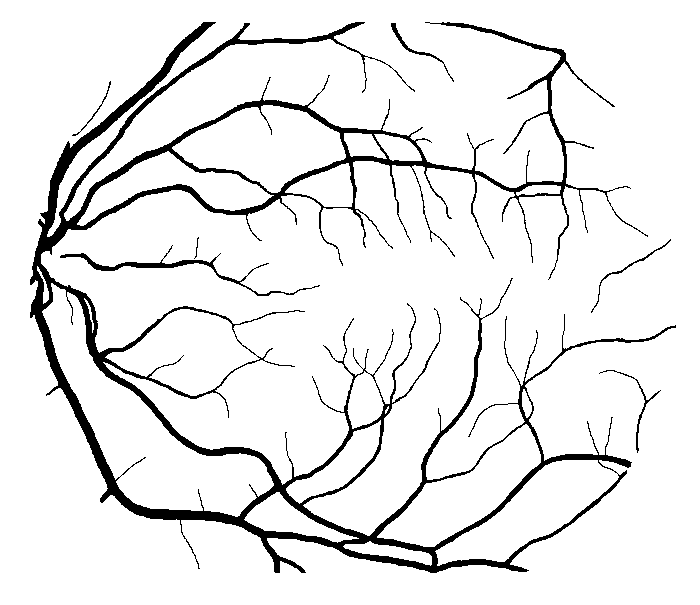
\includegraphics[width=6.4cm]{Figuras/Cap4/Stare_Manual_1}}
    \subfigure[\label{Fig:imgsoares1}]
        {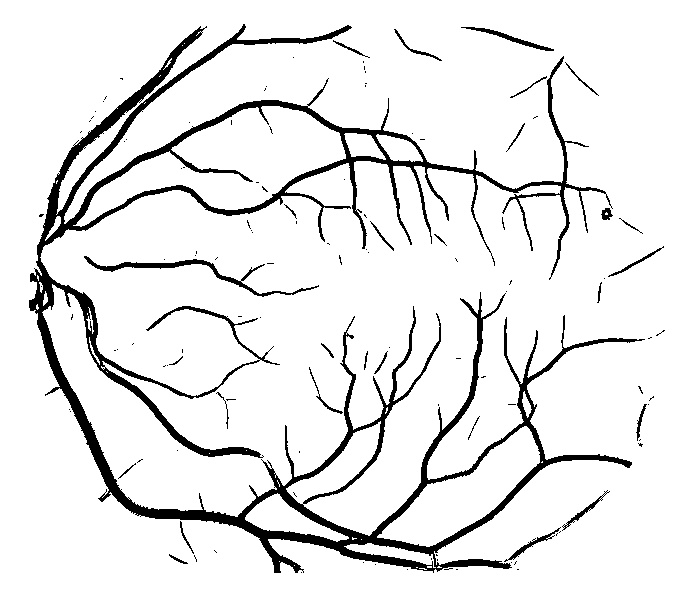
\includegraphics[width=6.4cm]{Figuras/Cap4/Stare_Soares_1}}
    \subfigure[\label{Fig:imgzana1}]
        {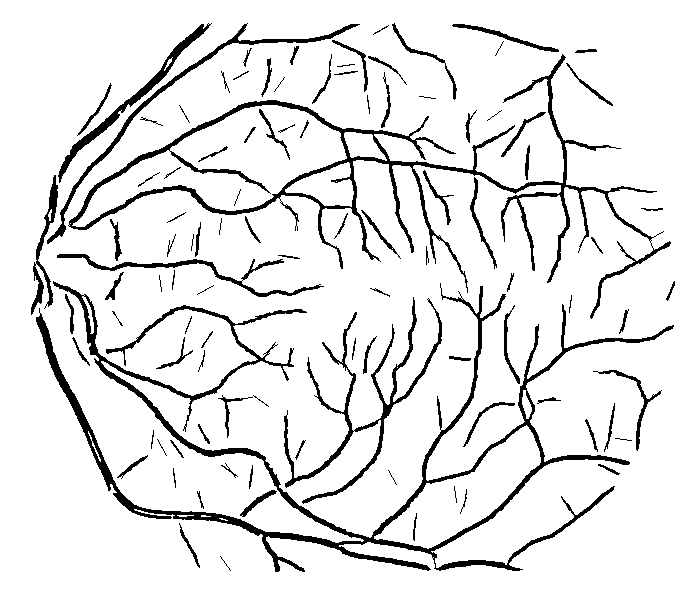
\includegraphics[width=6.4cm]{Figuras/Cap4/Stare_Zana_1}}
    \subfigure[\label{Fig:imgsoares1manual}]
        {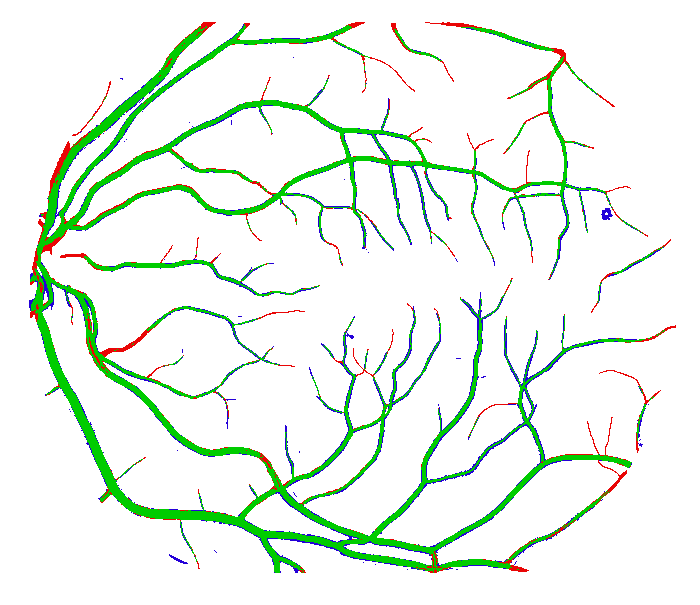
\includegraphics[width=6.4cm]{Figuras/Cap4/Stare_SoaresxManual_1}}
    \subfigure[\label{Fig:imgzana1manual}]
        {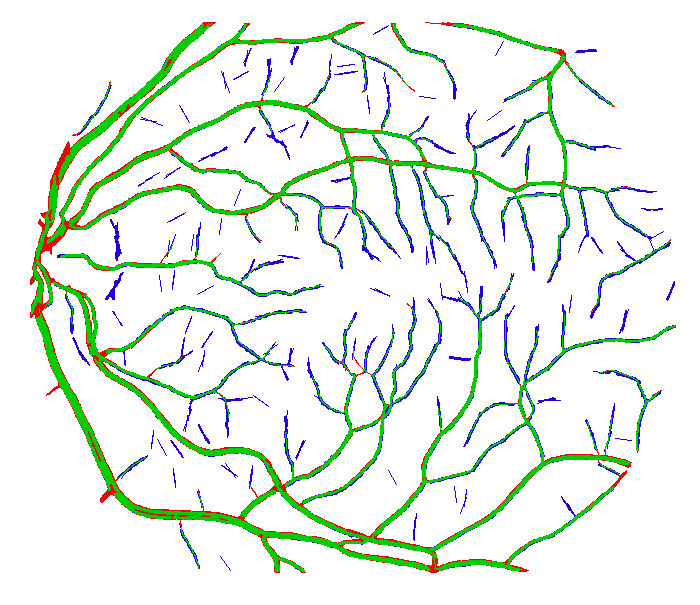
\includegraphics[width=6.4cm]{Figuras/Cap4/Stare_ZanaxManual_1}}
    \caption{(a) Imagem original (Fonte: Base de Dados STARE); (b) Mapa de refer\^{e}ncia (Fonte: Base de Dados STARE); (c) Imagem segmentada para o m\'{e}todo supervisionado (Fonte: Pr\'{o}prio Author); (d) Imagem segmentada para o m\'{e}todo n\~{a}o-supervisionado (Fonte: Pr\'{o}prio Author); (e) Imagem de compara\c{c}\~{a}o entre o m\'{e}todo supervisionado e o mapa de refer\^{e}ncia (Fonte: Pr\'{o}prio Author); (f) Imagem de compara\c{c}\~{a}o entre o m\'{e}todo n\~{a}o-supervisionado e o mapa de refer\^{e}ncia (Fonte: Pr\'{o}prio Author).}
    \label{Fig:exemplesStare}
\end{figure}

Diferentemente do que acontece na base DRIVE, o m\'{e}todo supervisionado apresenta desempenho superior para todas as medidas na base STARE. As Figuras \ref{Fig:exemplesStare}(e) e \ref{Fig:exemplesStare}(f) ilustram o desempenho dos m\'{e}todos na base STARE. Analogamente ao que acontece na base anterior, \'{e} poss\'{i}vel notar que o m\'{e}todo supervisionado possui uma quantidade inferior de pixels vermelhos, indicando melhor detec\c{c}\~{a}o de pixels de vasos. Contudo, o mesmo n\~{a}o \'{e} notado quando observamos a presen\c{c}a de pixels azuis. Para a base STARE, o m\'{e}todo supervisionado possui uma quantidade inferior de pixels erroneamente segmentados como vasos (pixels azuis), o que justifica seu desempenho superior com rela\c{c}\~{a}o \`{a} especificidade. Considerando os valores superiores de sensibilidade e especificidade, \'{e} esperado que a precis\~{a}o do m\'{e}todo supervisionado seja igualmente superior. De fato, a Tabela \ref{tabRESULTS} confirma esta expectativa.

\begin{table}[h]
  \caption{Valores m\'{e}dios para os resultados quantitativos para a base DRIVE.}
  \label{tabDRIVE}
  \centering
  \scalebox {0.85 }[0.85 ]{ 
    \begin{tabular}{llllll}
      \toprule
      M\'{e}todo & $Sb$ & $Ep$ & $Pc$\\
      \midrule                 
      \citeauthor{Zana:2001} (\citeyear{Zana:2001}) &0.6548 &\textbf{0.9803} &0.9377\\

      \citeauthor{Soares:2006} (\citeyear{Soares:2006}) &\textbf{0.7410} &0.9773 &\textbf{0.9464}\\

      \bottomrule
    \end{tabular}
  }
\end{table}

\begin{table}[h]
  \caption{Valores m\'{e}dios para os resultados quantitativos para a base STARE.}
  \label{tabRESULTS}
  \centering
  \scalebox {0.85 }[0.85 ]{ 
    \begin{tabular}{llllll}
      \toprule
      M\'{e}todo & $Sb$ & $Ep$ & $Pc$ \\
      \midrule                 
      \citeauthor{Zana:2001} (\citeyear{Zana:2001})  &0.7084 &0.9734 &0.9459 \\

      \citeauthor{Soares:2006} (\citeyear{Soares:2006})   &\textbf{0.7406} &\textbf{0.9790} & \textbf{0.9539} \\
      \bottomrule
    \end{tabular}
  }
\end{table}

A an\'{a}lise dos resultados das Tabelas \ref{tabDRIVE} e \ref{tabRESULTS} se referem \`{a} avalia\c{c}\~{a}o quantitativa dos m\'{e}todos. Entretanto, faz-se necess\'{a}rio avaliar a morfologia dos vasos, segundo atributos de conectividade, \'{a}rea e comprimento de vasos.

As Tabelas \ref{tabQLDRIVE} e \ref{tabQLSTARE} apresentam os valores m\'{e}dios das medidas de avalia\c{c}\~{a}o dos atributos morfol\'{o}gicos para as bases DRIVE e STARE, respectivamente. No geral, estes resultados comprovam a superioridade do m\'{e}todo supervisionado apontada pelas medidas de informa\c{c}\~{a}o quantitativa, mas existem alguns pontos importantes que ser\~{a}o detalhados a seguir. Os valores de \'{a}rea e comprimento s\~{a}o superiores para o m\'{e}todo supervisionado em ambas as bases. As Figuras \ref{Fig:exemplesArea} e \ref{Fig:exemplesCOmp} ilustram esses resultados. Para o primeiro caso, as imagens mostram uma diferen\c{c}a significativa de pixels vermelhos em vasos calibrosos do m\'{e}todo n\~{a}o-supervisionado. Este fato mostra que houve uma segmenta\c{c}\~{a}o de \'{a}rea inferior ao tamanho considerado correto. Apesar da sobre-segmenta\c{c}\~{a}o de \'{a}rea em alguns pontos de fronteiras de vasos do m\'{e}todo supervisionado, h\'{a} uma sub-segmenta\c{c}\~{a}o equivalente nas regi\~{o}es mais externas dos vasos na imagem do m\'{e}todo n\~{a}o-supervisionado. Ao final, a \'{a}rea inferior da imagem do m\'{e}todo n\~{a}o-supervisionado define seus valores menores para este atributo nas duas bases. A Figura \ref{Fig:exemplesCOmp} evidencia uma quantidade consideravelmente superior de pixels erroneamente detectados como vasos nas extremidades dos vasos do m\'{e}todo n\~{a}o-supervisionado. Assim, os vasos adquirem um comprimento superior ao seu comprimento original, evidenciando os valores de comprimento menor deste m\'{e}todo para as duas bases.

\begin{table}[h!]
  \caption{Valores m\'{e}dios para os resultados dos avaliadores de atributos morfol\'{o}gicos para base DRIVE.}
  \label{tabQLDRIVE}
  \centering
  \scalebox {0.85 }[0.85 ]{ 
    \begin{tabular}{lllll}
      \toprule
      M\'{e}todo & $C$ & $A$ & $L$ \\
      \midrule                 
      \citeauthor{Zana:2001} (\citeyear{Zana:2001}) &0.9928 &0.8931 &0.8531 \\

      \citeauthor{Soares:2006} (\citeyear{Soares:2006}) &\textbf{0.9938} &\textbf{0.9092} &\textbf{0.8769}\\

      \bottomrule
    \end{tabular}
  }
\end{table}

\begin{table}[h!]
  \caption{Valores m\'{e}dios para os resultados dos avaliadores de atributos morfol\'{o}gicos para base STARE.}
  \label{tabQLSTARE}
  \centering
  \scalebox {0.85 }[0.85 ]{ 
    \begin{tabular}{lllll}
      \toprule
      M\'{e}todo & $C$ & $A$ & $L$ \\
      \midrule                 
      \citeauthor{Zana:2001} (\citeyear{Zana:2001})  &\textbf{0.9960} &0.8676 &0.8568 \\

      \citeauthor{Soares:2006} (\citeyear{Soares:2006}) &0.9946 &\textbf{0.8821} &\textbf{0.8779} \\
      \bottomrule
    \end{tabular}
  }
\end{table}

Analogamente ao que acontece para a especificidade, a conectividade dos vasos difere entre os resultados de segmenta\c{c}\~{a}o pelos 2 m\'{e}todos. O m\'{e}todo n\~{a}o-supervisionado apresenta resultado melhor para a base STARE. J\'{a} o m\'{e}todo supervisionado possui valor de conectividade superior para a base DRIVE. As Figuras \ref{Fig:exemplesConDrive} e \ref{Fig:exemplesConStare} ilustram o desempenho dos m\'{e}todos para uma imagem de cada base. Analisando as Figuras \ref{Fig:exemplesConDrive}(d) e \ref{Fig:exemplesConDrive}(f), pode-se perceber que h\'{a} uma maior fragmenta\c{c}\~{a}o dos vasos na imagem do m\'{e}todo n\~{a}o-supervisionado, confirmando os resultados apresentados na Tabela \ref{tabQLDRIVE}. Esta fragmenta\c{c}\~{a}o pode ser vista pela quantidade elevada de pixels vermelhos localizados em regi\~{o}es de liga\c{c}\~{a}o dos vasos. Estes pixels indicam que n\~{a}o houve segmenta\c{c}\~{a}o nessas regi\~{o}es, o que torna os vasos desconectados. Em contrapartida, a an\'{a}lise das Figuras \ref{Fig:exemplesConStare}(d) e \ref{Fig:exemplesConStare}(f) permite afirmar que a rede do m\'{e}todo supervisionado possui uma fragmenta\c{c}\~{a}o superior para a base STARE. Contudo, esta fragmenta\c{c}\~{a}o difere do modelo de fragmenta\c{c}\~{a}o anterior, pois esta decorre da quebra dos vasos ao longo de seu comprimento. Assim, pequenos fragmentos de vasos s\~{a}o vistos onde deveria haver apenas um \'{u}nico vaso conectado. 

Considerando uma an\'{a}lise global de cada um dos m\'{e}todos, \'{e} poss\'{i}vel determinar que o m\'{e}todo supervisionado identifica uma rede maior e melhor conectada. Esse fato \'{e} comprovado pelos maiores valores das medidas deste m\'{e}todo para a maioria das bases. Portanto, os valores obtidos para as medidas permitem comprovar que o m\'{e}todo supervisionado detecta uma quantidade maior de vasos \'{e} detectada e essa detec\c{c}\~{a}o possui, no geral, vasos mais conectados, vasos com melhor estimativa de \'{a}rea e vasos de comprimentos mais coerentes dentro da rede.


\begin{figure}[!h]
    \centering
    \subfigure[\label{Fig:imgrgb17Drive}]
        {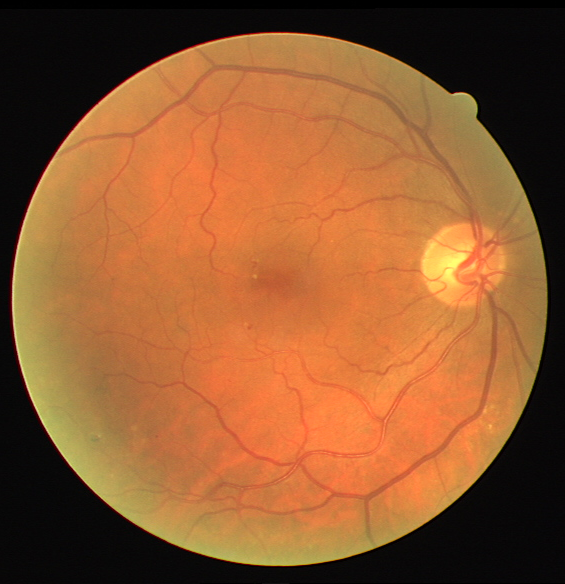
\includegraphics[width=6cm]{Figuras/Cap4/Drive_RGB_Area_17}}
    \subfigure[\label{Fig:imgmanual17Drive}]
        {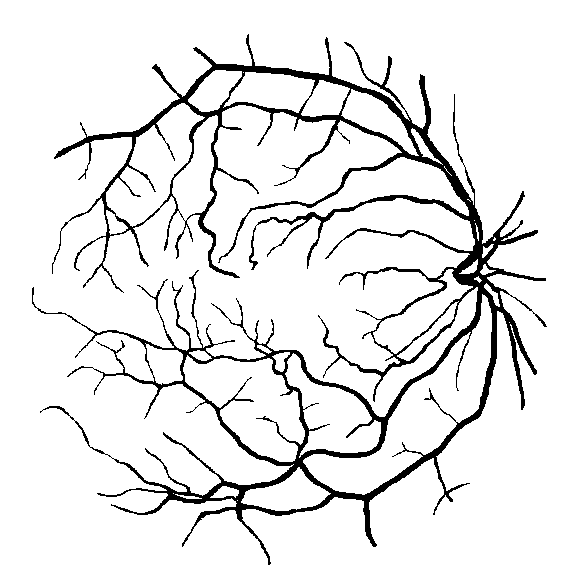
\includegraphics[width=6cm]{Figuras/Cap4/Drive_Manual_Area_17}}
    \subfigure[\label{Fig:imgsoares17Drive}]
        {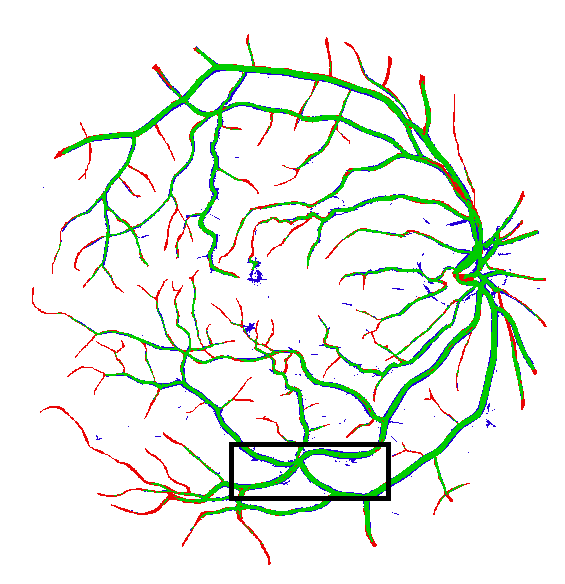
\includegraphics[width=6cm]{Figuras/Cap4/Drive_Soares_Area_17}}
    \subfigure[\label{Fig:imgzana17Drive}]
        {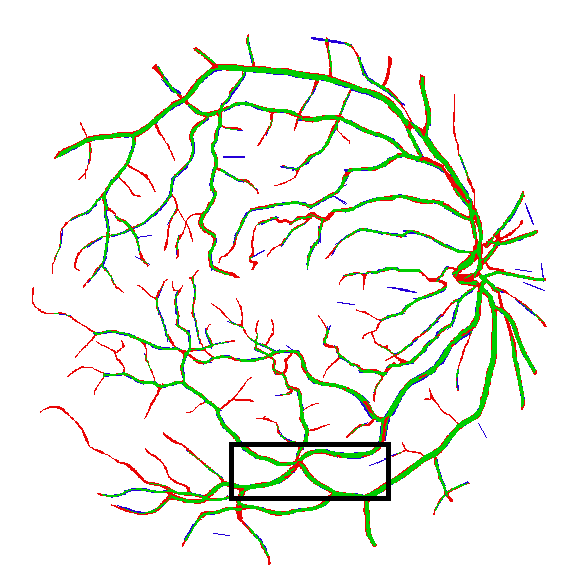
\includegraphics[width=6cm]{Figuras/Cap4/Drive_Zana_Area_17}}
    \subfigure[\label{Fig:imgsoares17manualDrive}]
        {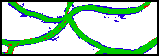
\includegraphics[width=6cm]{Figuras/Cap4/Drive_Cut_Soares_Area_17}}
    \subfigure[\label{Fig:imgzana17manualDrive}]
        {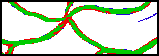
\includegraphics[width=6cm]{Figuras/Cap4/Drive_Cut_Zana_Area_17}}
    \caption{(a) Imagem original (Fonte: Base de Dados DRIVE); (b) Mapa de refer\^{e}ncia (Fonte: Base de Dados DRIVE); (c) Imagem de compara\c{c}\~{a}o entre o m\'{e}todo supervisionado e o mapa de refer\^{e}ncia com sub-regi\~{a}o destacada (Fonte: Pr\'{o}prio Author); (d) Imagem de compara\c{c}\~{a}o entre o m\'{e}todo n\~{a}o-supervisionado e o mapa de refer\^{e}ncia com sub-regi\~{a}o destacada (Fonte: Pr\'{o}prio Author); (e) Sub-regi\~{a}o ampliada da imagem de compara\c{c}\~{a}o para o m\'{e}todo supervisionado (Fonte: Pr\'{o}prio Autor); (f) Sub-regi\~{a}o ampliada da imagem de compara\c{c}\~{a}o para o m\'{e}todo n\~{a}o-supervisionado (Fonte: Pr\'{o}prio Autor).}
    \label{Fig:exemplesArea}
\end{figure}

\begin{figure}[!h]
    \centering
    \subfigure[\label{Fig:imgrgb9Stare}]
        {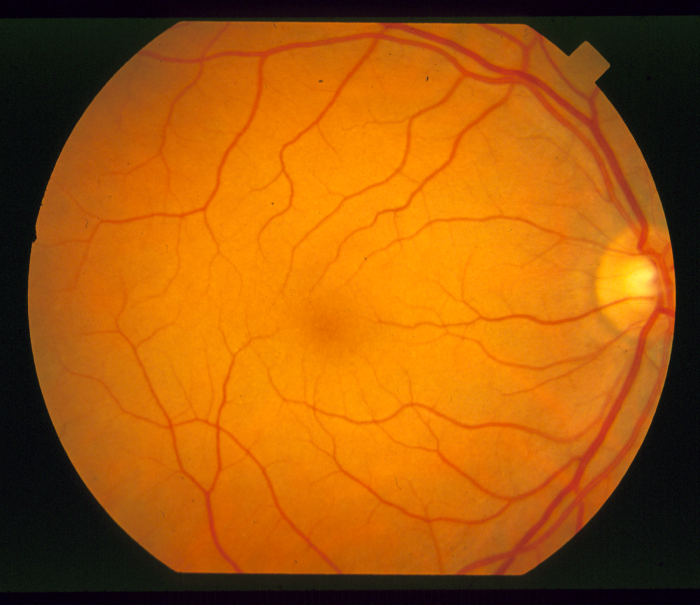
\includegraphics[width=6cm]{Figuras/Cap4/Stare_RGB_Comp_9}}
    \subfigure[\label{Fig:imgmanual9Stare}]
        {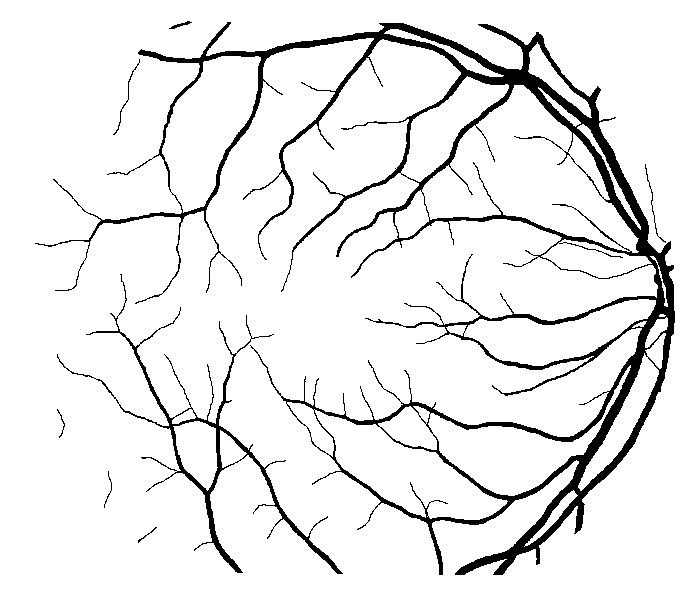
\includegraphics[width=6cm]{Figuras/Cap4/Stare_Manual_Comp_9}}
    \subfigure[\label{Fig:imgsoares9Stare}]
        {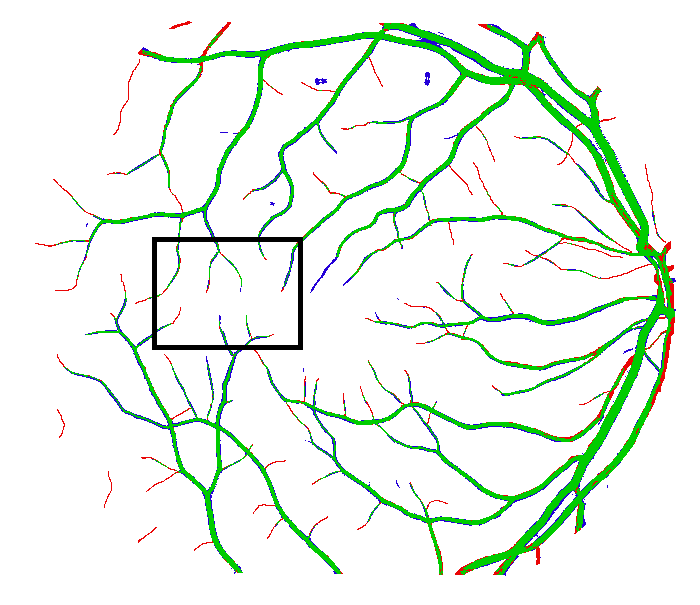
\includegraphics[width=6cm]{Figuras/Cap4/Stare_Soares_Comp_9}}
    \subfigure[\label{Fig:imgzana9Stare}]
        {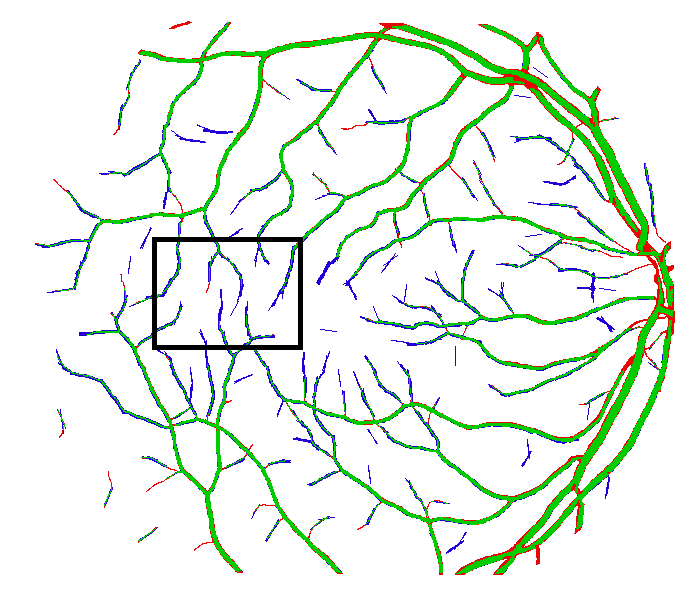
\includegraphics[width=6cm]{Figuras/Cap4/Stare_Zana_Comp_9}}
    \subfigure[\label{Fig:imgsoares9manualStare}]
        {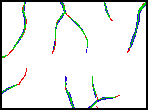
\includegraphics[width=6cm]{Figuras/Cap4/Stare_Cut_Soares_Comp_9}}
    \subfigure[\label{Fig:imgzana9manualStare}]
        {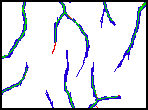
\includegraphics[width=6cm]{Figuras/Cap4/Stare_Cut_Zana_Comp_9}}
    \caption{(a) Imagem original (Fonte: Base de Dados STARE); (b) Mapa de refer\^{e}ncia (Fonte: Base de Dados STARE); (c) Imagem de compara\c{c}\~{a}o entre o m\'{e}todo supervisionado e o mapa de refer\^{e}ncia com sub-regi\~{a}o destacada (Fonte: Pr\'{o}prio Author); (d) Imagem de compara\c{c}\~{a}o entre o m\'{e}todo n\~{a}o-supervisionado e o mapa de refer\^{e}ncia com sub-regi\~{a}o destacada (Fonte: Pr\'{o}prio Author); (e) Sub-regi\~{a}o ampliada da imagem de compara\c{c}\~{a}o para o m\'{e}todo supervisionado (Fonte: Pr\'{o}prio Autor); (f) Sub-regi\~{a}o ampliada da imagem de compara\c{c}\~{a}o para o m\'{e}todo n\~{a}o-supervisionado (Fonte: Pr\'{o}prio Autor).}
    \label{Fig:exemplesCOmp}
\end{figure}

\begin{figure}[!h]
    \centering
    \subfigure[\label{Fig:imgrgb10Drive}]
        {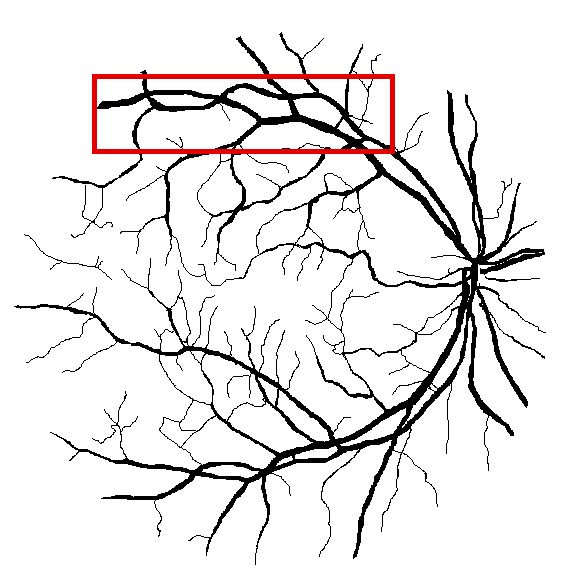
\includegraphics[width=6cm]{Figuras/Cap4/Drive_Manual_Con_10}}
    \subfigure[\label{Fig:imgmanual10Drive}]
        {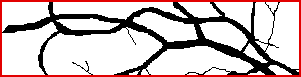
\includegraphics[width=6.5cm, trim = 0cm -3.5cm 0cm 0cm]{Figuras/Cap4/Drive_Manual_Cut_Con_10}}
    \subfigure[\label{Fig:imgsoares10Drive}]
        {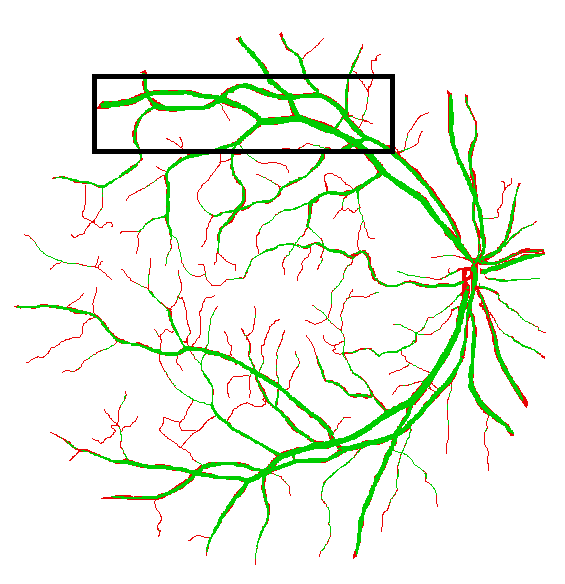
\includegraphics[width=6cm]{Figuras/Cap4/Drive_Soares_Con_10}}
    \subfigure[\label{Fig:imgzana10Drive}]
        {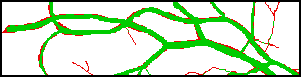
\includegraphics[width=6.5cm, trim = 0cm -3.5cm 0cm 0cm]{Figuras/Cap4/Drive_Soares_Cut_Con_10}}
    \subfigure[\label{Fig:imgsoares10manualDrive}]
        {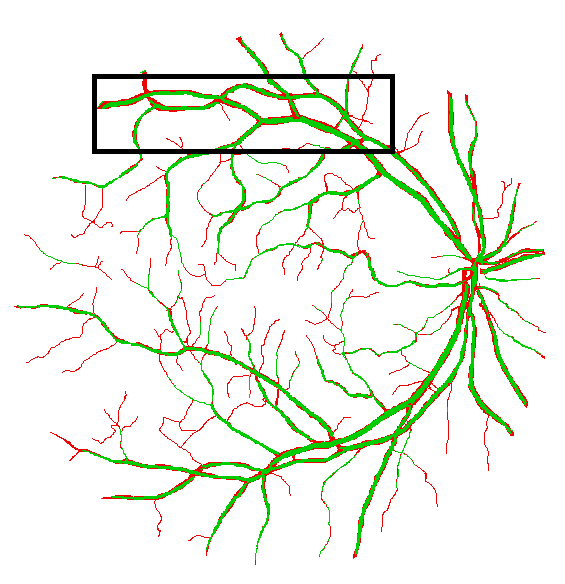
\includegraphics[width=6cm]{Figuras/Cap4/Drive_Zana_Con_10}}
    \subfigure[\label{Fig:imgzana10manualDrive}]
        {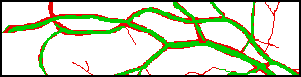
\includegraphics[width=6.5cm, trim = 0cm -3.5cm 0cm 0cm]{Figuras/Cap4/Drive_Zana_Cut_Con_10}}
    \caption{(a) Mapa de refer\^{e}ncia com sub-regi\~{a}o em destaque (Fonte: Base de Dados DRIVE); (b) Sub-regi\~{a}o ampliada do mapa de refer\^{e}ncia (Fonte: Base de Dados DRIVE); (c) Imagem de compara\c{c}\~{a}o para m\'{e}todo supervisionado com sub-regi\~{a}o em destaque (Fonte: Pr\'{o}prio Author); (d) Sub-regi\~{a}o ampliada dda imagem de compara\c{c}\~{a}o para o m\'{e}todo supervisionado (Fonte: Pr\'{o}prio Author); (e) Imagem de compara\c{c}\~{a}o para m\'{e}todo n\~{a}o-supervisionado com sub-regi\~{a}o em destaque (Fonte: Pr\'{o}prio Author); (f) Sub-regi\~{a}o ampliada dda imagem de compara\c{c}\~{a}o para o m\'{e}todo n\~{a}o-supervisionado (Fonte: Pr\'{o}prio Author);.}
    \label{Fig:exemplesConDrive}
\end{figure}


\begin{figure}[!h]
    \centering
    \subfigure[\label{Fig:imgrgb10Drive}]
        {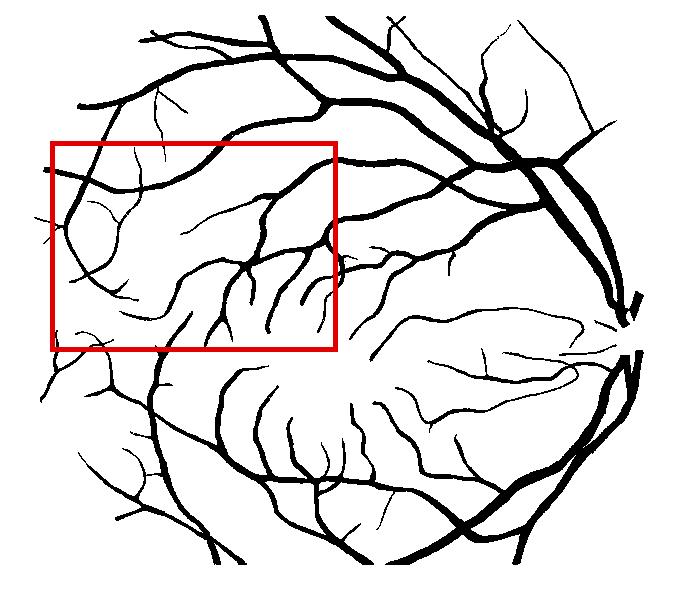
\includegraphics[width=6cm]{Figuras/Cap4/Stare_Manual_Con_16}}
    \subfigure[\label{Fig:imgmanual10Drive}]
        {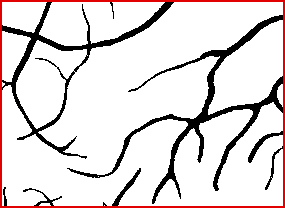
\includegraphics[width=6.5cm]{Figuras/Cap4/Stare_Manual_Cut_Con_16}}
    \subfigure[\label{Fig:imgsoares10Drive}]
        {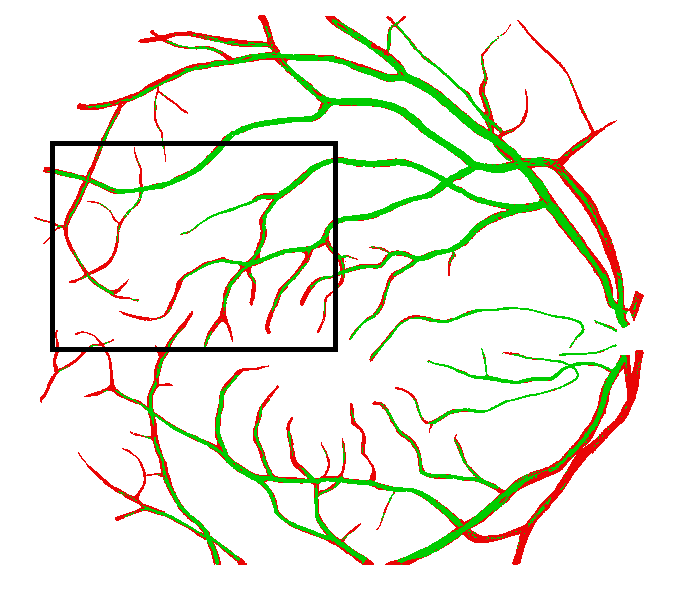
\includegraphics[width=6cm]{Figuras/Cap4/Stare_Soares_Con_16}}
    \subfigure[\label{Fig:imgzana10Drive}]
        {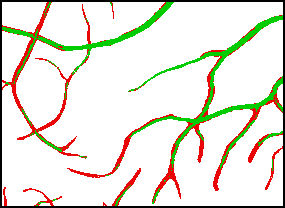
\includegraphics[width=6.5cm]{Figuras/Cap4/Stare_Soares_Cut_Con_16}}
    \subfigure[\label{Fig:imgsoares10manualDrive}]
        {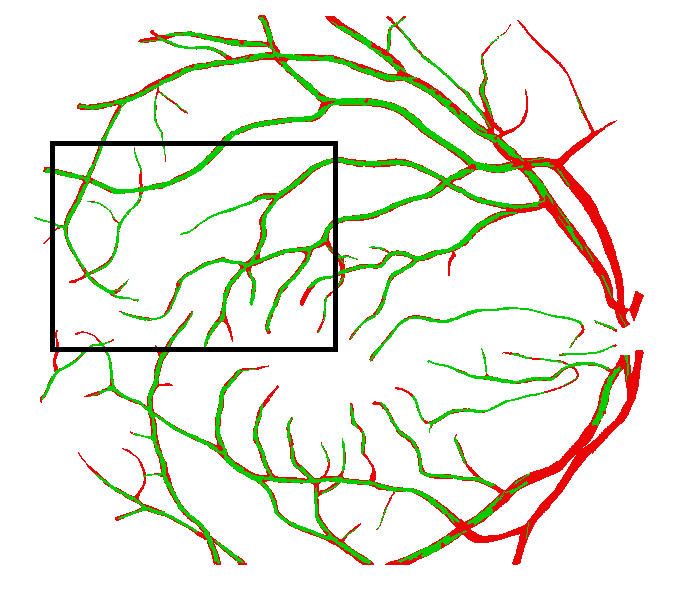
\includegraphics[width=6cm]{Figuras/Cap4/Stare_Zana_Con_16}}
    \subfigure[\label{Fig:imgzana10manualDrive}]
        {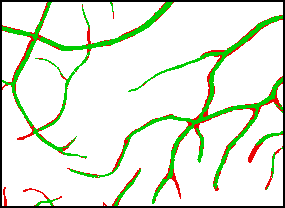
\includegraphics[width=6.5cm]{Figuras/Cap4/Stare_Zana_Cut_Con_16}}
    \caption{(a) Mapa de refer\^{e}ncia com sub-regi\~{a}o em destaque (Fonte: Base de Dados STARE); (b) Sub-regi\~{a}o ampliada do mapa de refer\^{e}ncia (Fonte: Base de Dados STARE); (c) Imagem de compara\c{c}\~{a}o para m\'{e}todo supervisionado com sub-regi\~{a}o em destaque (Fonte: Pr\'{o}prio Author); (d) Sub-regi\~{a}o ampliada dda imagem de compara\c{c}\~{a}o para o m\'{e}todo supervisionado (Fonte: Pr\'{o}prio Author); (e) Imagem de compara\c{c}\~{a}o para m\'{e}todo n\~{a}o-supervisionado com sub-regi\~{a}o em destaque (Fonte: Pr\'{o}prio Author); (f) Sub-regi\~{a}o ampliada dda imagem de compara\c{c}\~{a}o para o m\'{e}todo n\~{a}o-supervisionado (Fonte: Pr\'{o}prio Author);.}
    \label{Fig:exemplesConStare}
\end{figure}

